\documentclass[journal]{IEEEtran}
\usepackage{amsmath,amsfonts}
\usepackage{algorithmic}
\usepackage{algorithm}
\usepackage{amssymb}
\usepackage{array}
\usepackage[caption=false,font=normalsize,labelfont=sf,textfont=sf]{subfig}
\usepackage{textcomp}
\usepackage{stfloats}
\usepackage{url}
\usepackage{verbatim}
\usepackage{graphicx}
\usepackage{cite}
\usepackage{xcolor}
\hyphenation{op-tical net-works semi-conduc-tor IEEE-Xplore}

% updated with editorial comments 8/9/2021
% not show the red box
\usepackage[hidelinks]{hyperref}

\usepackage{booktabs} % for \hline
\renewcommand{\algorithmicrequire}{\textbf{Input:}}
\renewcommand{\algorithmicensure}{\textbf{Output:}}
\usepackage{threeparttable}
\usepackage{amsthm}
\newtheorem{definition}{Definition}
\newtheorem{proposition}{Proposition}
\usepackage{listings}

\begin{document}

\title{Efficient Implementations of SPHINCS\textsuperscript{+} on GPUs}

\author{Jiahao Xiang and Lang Li.
  % <-this % stops a space

  \thanks{This work is supported by the Hunan Provincial Natural Science Foundation of China (2022JJ30103), Postgraduate Scientific Research Innovation Project of Hunan Province (CX20240977), “the 14th Five-Year Plan” Key Disciplines and Application-oriented Special Disciplines of Hunan Province (Xiangjiaotong [2022] 351), the Science and Technology Innovation Program of Hunan Province (2016TP1020).}

  \thanks{Jiahao Xiang and Lang Li are with the Hunan Provincial Key Laboratory of Intelligent Information Processing and Application, Hengyang Normal University, Hengyang 421002, China, and also with the College of Computer Science and Technology, Hengyang Normal University, Hengyang 421002, China (e-mail: jiahaoxiang2000@gmail.com; lilang911@126.com).}% <-this % stops a space
}
% \thanks{Manuscript received April 19, 2021; revised August 16, 2021.}}
% \thanks{Manuscript received }}

% The paper headers
\markboth{Journal of \LaTeX\ Class Files,~Vol.~14, No.~8, August~2021}%
{Shell \MakeLowercase{\textit{et al.}}: A Sample Article Using IEEEtran.cls for IEEE Journals}

\IEEEpubid{}
% Remember, if you use this you must call \IEEEpubidadjcol in the second
% column for its text to clear the IEEEpubid mark.

\maketitle

\begin{abstract}
  \textcolor{blue}{
    The Post-Quantum Cryptography (PQC) standardization process has led to the development of SPHINCS\textsuperscript{+}, a stateless hash-based signature scheme that provides long-term security. The high computational cost of SPHINCS\textsuperscript{+} has motivated research into efficient implementations on various platforms. In this work, we present a GPU-based implementation of SPHINCS\textsuperscript{+} that achieves high throughput while maintaining security guarantees. Our implementation leverages the parallel processing capabilities of GPUs to accelerate the signature generation process. We evaluate the performance of our implementation on an NVIDIA RTX 4090 GPU and demonstrate that it can achieve a throughput of xxx for the SPHINCS\textsuperscript{+} signature generation. Our results show that GPUs can be an effective platform for accelerating SPHINCS\textsuperscript{+} and other post-quantum cryptographic schemes.
  }

\end{abstract}

\begin{IEEEkeywords}
  Software implementation, GPU, signature algorithm.
\end{IEEEkeywords}

\section{Introduction}
\label{sec:intro}

% Growing data volumes necessitate high-throughput encryption schemes to ensure data confidentiality. The Advanced Encryption Standard (AES) remains the most prominent block cipher, with software implementations commonly adopted for flexibility and scalability.

\color{blue}

\IEEEPARstart{T}{he} quantum computers leverage quantum-mechanical phenomena to process data, raising significant concerns about the resilience of classical cryptographic methods. 
The security offered by widely deployed public-key cryptosystems, such as RSA and ECC, is jeopardized by Shor's algorithm \cite{Shor1994}, motivating comprehensive research on alternative cryptographic solutions. In response, the National Institute of Standards and Technology (NIST) initiated the Post-Quantum Cryptography (PQC) standardization process to develop novel schemes that withstand quantum computing capabilities \cite{NIST2016}.

SPHINCS\textsuperscript{+} is a representative stateless hash-based signature scheme and a finalist in the ongoing NIST standardization effort \cite{Turan}. Long-term security against advanced quantum attacks is targeted by employing robust cryptographic hash functions \cite{Bernstein2019}. The high computational cost of SPHINCS\textsuperscript{+} has motivated further investigations into efficient implementations across CPUs, FPGAs, and GPUs \cite{Joseph2022} to facilitate smooth adoption by organizations transitioning to post-quantum cryptography.

\subsection{Related Work}

\subsection{Motivation}

\subsection{Contributions}

\color{black}

% \section*{Acknowledgments}

% {\appendix[Proof of the Zonklar Equations]
% Use $\backslash${\tt{appendix}} if you have a single appendix:
% Do not use $\backslash${\tt{section}} anymore after $\backslash${\tt{appendix}}, only $\backslash${\tt{section*}}.
% If you have multiple appendixes use $\backslash${\tt{appendices}} then use $\backslash${\tt{section}} to start each appendix.
% You must declare a $\backslash${\tt{section}} before using any $\backslash${\tt{subsection}} or using $\backslash${\tt{label}} ($\backslash${\tt{appendices}} by itself
%  starts a section numbered zero.)}

%{\appendices
%\section*{Proof of the First  Equation}
%Appendix one text goes here.
% You can choose not to have a title for an appendix if you want by leaving the argument blank
%\section*{Proof of the Second  Equation}
%Appendix two text goes here.}

% argument is your BibTeX string definitions and bibliography database(s)
\bibliography{biblio}

\bibliographystyle{IEEEtran}

% \newpage

% \bf{If you include a photo:}\vspace{-33pt}
\begin{IEEEbiography}[{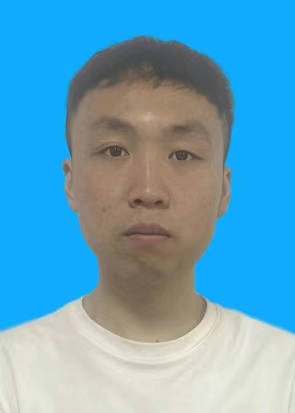
\includegraphics[width=1in,height=1.25in,clip,keepaspectratio]{./fig/slef.jpg}}]{Jiahao Xiang}
  is pursuing a Master's degree in Electronic Information at Hengyang Normal University, China. His research focuses on cryptographic engineering and efficient implementations of block ciphers on resource-constrained devices. Publications include works on lightweight cryptography optimization and contributions to open-source cryptographic projects.
\end{IEEEbiography}

\begin{IEEEbiography}[{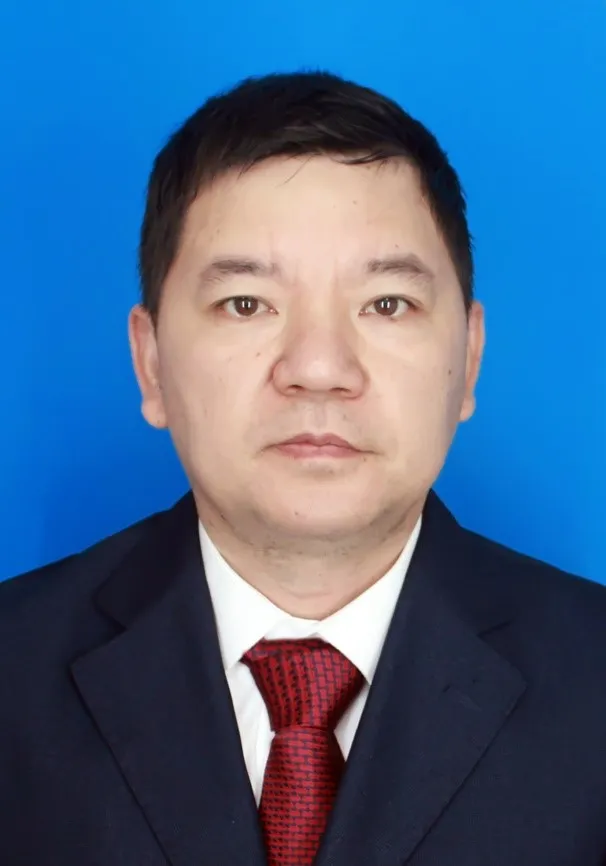
\includegraphics[width=1in,height=1.25in,clip,keepaspectratio]{./fig/boss.png}}]{Lang Li}
  received his Ph.D. and Master's degrees in computer science from Hunan University, Changsha, China, in 2010 and 2006, respectively, and earned his B.S. degree in circuits and systems from Hunan Normal University in 1996. Since 2011, he has been working as a professor in the College of Computer Science and Technology at the Hengyang Normal University, Hengyang, China. He has research interests in embedded system and information security.
\end{IEEEbiography}

% \vspace{11pt}

% \bf{If you will not include a photo:}\vspace{-33pt}
% \begin{IEEEbiographynophoto}{Jiahao Xiang}
% is pursuing a Master's degree in Electronic Information at Hengyang Normal University, China. His research focuses on cryptographic engineering and efficient implementations of block ciphers on resource-constrained devices. Publications include works on lightweight cryptography optimization and contributions to open-source cryptographic projects.
% \end{IEEEbiographynophoto}

% \begin{IEEEbiographynophoto}{Lang Li}
%  received his Ph.D. and Master's degrees in computer science from Hunan University, Changsha, China, in 2010 and 2006, respectively, and earned his B.S. degree in circuits and systems from Hunan Normal University in 1996. Since 2011, he has been working as a professor in the College of Computer Science and Technology at the Hengyang Normal University, Hengyang, China. He has research interests in embedded system and information security.
% \end{IEEEbiographynophoto}

\vfill

\end{document}
